\chapter{Arquitectura}

La aplicación sigue una variación de la arquitectura de tres capas. Las capas
de presentación y dominio permanecen inalteradas. Sin embargo, esta aplicación
no necesita de almacenamiento externo, sino que se obtiene esta información
directamente del servidor. Por ese motivo, la capa de persistencia ha sido
sustituida por una capa de comunicaciones.

\begin{figure}[h]
\caption{Visión general de la arquitectura}
\centering
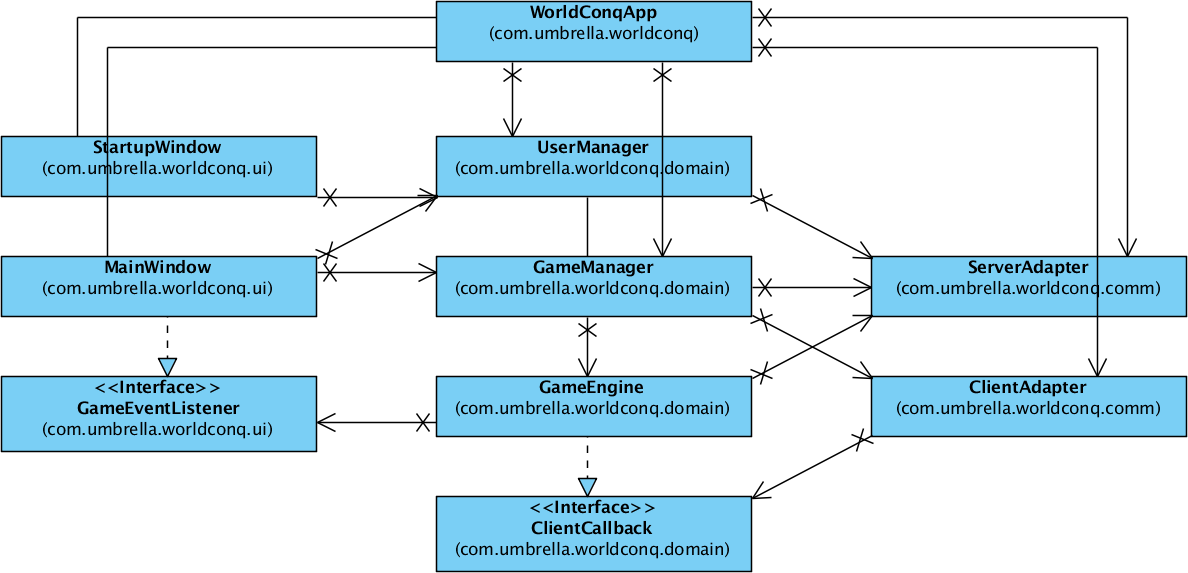
\includegraphics[scale=0.4]{img/ch02arch-overview.png}
\end{figure}

La visibilidad entre clases va de manera jerárquica, de manera que las clases
de presentación conocen a las de dominio, y las de dominio a las de
comunicaciones, pero no al revés. Para los casos en los que es necesario un
flujo de información en sentido contrario, se han creado interfaces para
desacoplar en la medida de los posible las capas inferiores.

La clase \texttt{WorldConqApp} es la única clase que no pertenece a ninguna de
las capas. Su función es la de ser el punto de entrada de la aplicación,
encargada de crear la estructura de clases, sus relaciones, y configurarlas a
partir de los parámetros de entrada.

\section{Capa de comunicaciones}

Esta capa contiene las clases \texttt{ServerAdapter} y \texttt{ClientAdapter}.
Ambas clases sirven de pasarela para los datos que fluyen entre el servidor y la
capa de dominio.

Estas clases incluyen una pequeña lógica de control. En el caso de la clase
\texttt{ServerAdapter}, ésta debe ser configurada con los datos del servidor
para así poder crear el \textit{proxy} a la interfaz remota. La ausencia de
esta configuración generará una excepción.

La clase \texttt{ClientAdapter} en cambio escucha todas las peticiones que
realiza el servidor sobre el cliente. Esta clase filtra estas peticiones de
acuerdo al juego activo en ese momento, descartando aquellas que no concuerden.

\section{Capa de dominio}

Esta capa está dividida en tres clases que se corresponden con los tres módulos
funcionales de la aplicación: gestión de usuarios, gestión de partidas, y motor
de juego.

La clase \texttt{UserManager} es la encargada de crear nuevas cuentas en la
aplicación y de mantener la información de la sesión activa. A esta clase
acceden el resto de clases para obtener la información sobre el jugador. De
manera análoga, la clase \texttt{GameManager} gestiona el listado, creación y
carga de partidas.

\begin{figure}[h]
\caption{Modelos de datos}
\centering
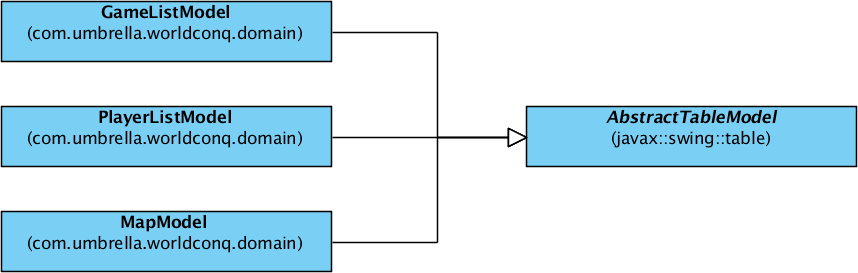
\includegraphics[scale=0.4]{img/ch02arch-models.png}
\end{figure}

Los datos de las partidas disponibles en el servidor son almacenados en objetos
de tipo \texttt{GameListModel}. Esta clase, y otras que se describen a
continuación, heredan de la clase \texttt{AbstractTableModel}. Esta clase
abstracta forma parte del \textit{framework} que proporciona Swing para
implementar el patrón arquitectónico Model-Vista-Controlador.

Hacer uso de este \textit{framework} significa que los accesos que hacen las
vistas a los modelos están definidos de antemano por una serie de interfaces.
Esto permite asociar clases disponibles en Swing con clases implementadas por el
equipo de trabajo de forma transparente.

En último lugar está el motor de juego, la clase \texttt{GameEngine}. Esta
clase se crea al comenzar a jugar a una partida e implementa toda la lógica de
dominio de una partida. Los datos con los que trabaja están almacenados en las
clases \texttt{PlayerListModel} y \texttt{MapModel}, los cuales heredan de la
clase \texttt{AbstractTableModel}, nombrada anteriormente.

\section{Capa de presentación}

En esta capa se encuentra la clase \texttt{StartupWindow}. Esta clase
representa a la primera ventana que se muestra. En ella, el usuario puede
registrar un nuevo usuario en el sistema y acceder con él.

Una vez accedido, se muestra la ventana principal, representada por la clase
\texttt{MainWindow}. Dentro de esta ventana existen dos modos de ejecución: el
modo de sala de espera y el modo partida.

\begin{figure}[h]
\caption{Vistas de datos}
\centering
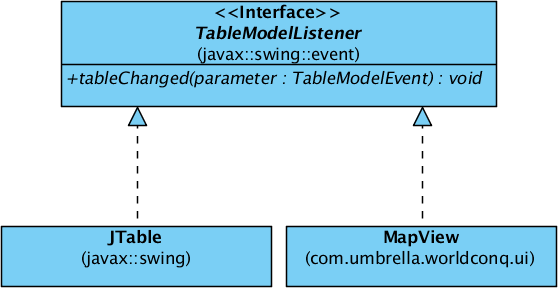
\includegraphics[scale=0.4]{img/ch02arch-views.png}
\end{figure}

En el modo de sala de espera, el usuario puede ver las partidas disponibles o
crear otras nuevas. Una vez se decida a cual jugar, la aplicación pasa a modo
partida.

La interfaz del modo partida se compone principalmente del mapa de juego. Junto
a él existen otro paneles informativos con los jugadores en la partida o una
lista con los últimos eventos.

Tanto las listas de partida como el mapa de juego implementan la interfaz
\texttt{TableModelListener}. Esto permite que estas clases puedan ser añadidas
como observadores de los cambios que sucedan en los modelos de datos.
